\documentclass{beamer}
\usepackage[utf8]{inputenc}
\usepackage{graphicx}
\usepackage{relsize}

\hypersetup{
    colorlinks,%
    citecolor=blue,%
    filecolor=blue,%
    linkcolor=blue,%
    urlcolor=blue 
    %urlcolor=mygreylink     % can put red here to better visualize the links
}

\author[Sowmya Vajjala]{Instructor: Sowmya Vajjala}

\title[LING 520]{LING 520: Computational Analysis of English}
\subtitle{Semester: FALL '16}

\date{29 September 2016}

\institute{Iowa State University, USA}
%%%%%%%%%%%%%%%%%%%%%%%%%%%

\begin{document}

\begin{frame}\titlepage
\end{frame}

\begin{frame}
\frametitle{Class outline}
\begin{itemize}
\item Assignment 2 Discussion
\item POS Tagging - Background
\item Rule based and Probabilistic POS tagging
\item Assignment 3 Description
\item Practice exercises
\end{itemize}
\end{frame}

\begin{frame}
\frametitle{Assignment 2 Discussion}
Volunteers needed.
\end{frame}

\begin{frame}
\frametitle{POS tagging Background-1}
\begin{itemize}
\item Task: tag every word in a sentence with its part of speech.
\item Used as a pre-processing task for a number of other NLP tasks. Also useful for doing corpus linguistic analysis
\item Problem 1: disambiguating which tag to use for a word in given context
\item Problem 2: how to adapt the tagger to different types and genres of data (news text, research articles speech, tweets etc.)
\end{itemize}
\end{frame}

\begin{frame}
\frametitle{POS tagging Background-2}
\begin{itemize}
\item Broadly 8 parts of speech described in Grammar classes - Noun, verb, adjective, adverb, pronoun, preposition, conjunction, interjection.
\item In NLP, they are slightly more fine-grained.
\item POS taggers for a language are developed based on the tagsets that are standardized for that language.
\item Tagsets are standardized by projects involving groups of linguists and computer scientists, usually in the early days of NLP research for a given language.
\item While all tagsets have some common features, there are also some language specific tags.
\end{itemize}
\end{frame}

\begin{frame}
\frametitle{Some POS Tagsets: English}
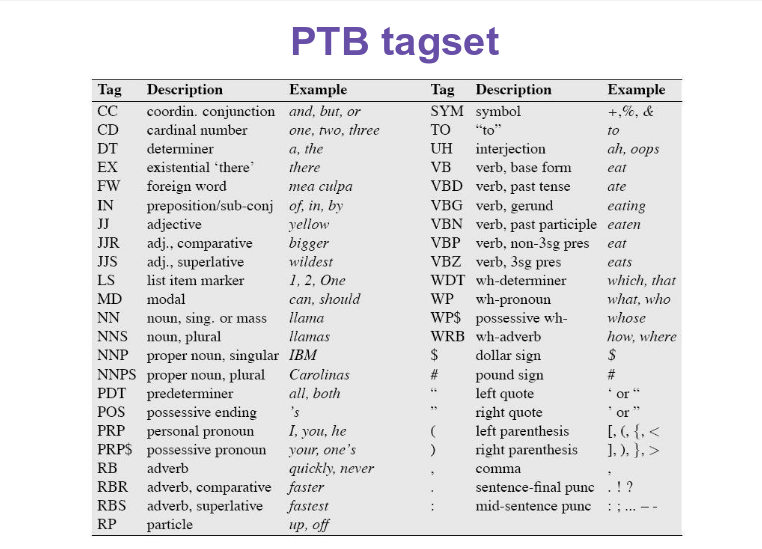
\includegraphics[width=0.9\textwidth]{posenglish.png}
\end{frame}

\begin{frame}
\frametitle{Other English Tagsets}
\begin{itemize}
\item Though PTB is the most commonly used tagset for English, there are some others too.
\item e.g., NUPOS tagset: \url{http://morphadorner.northwestern.edu/documentation/nupos/}
\item CLAWS7 tagset: \url{http://ucrel.lancs.ac.uk/claws/}
\end{itemize}
\end{frame}

\begin{frame}
\frametitle{Some POS Tagsets: German}
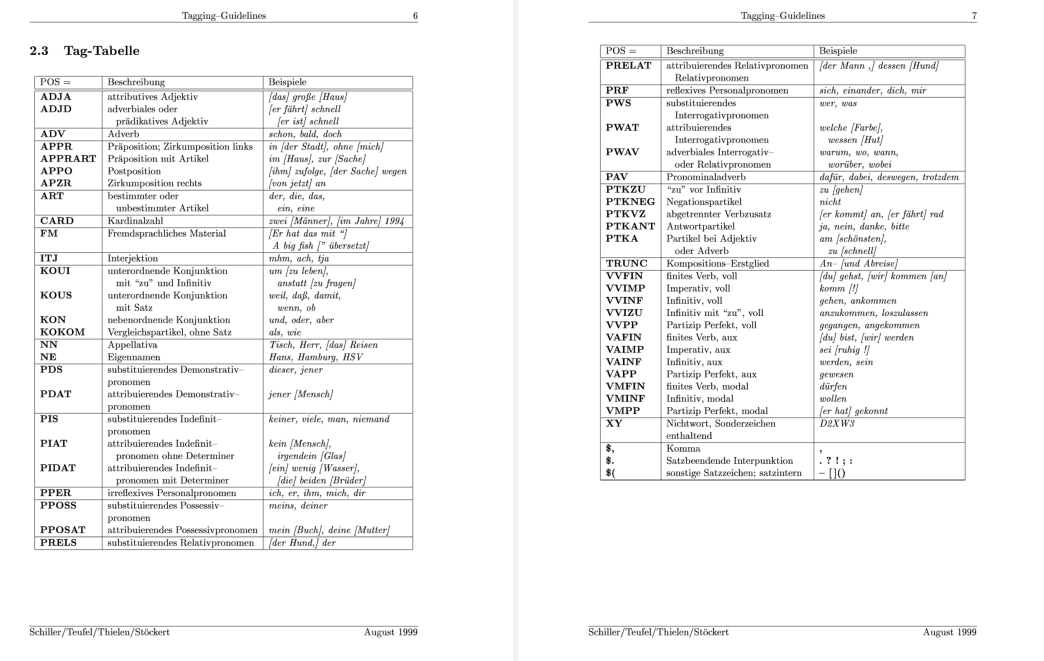
\includegraphics[width=0.9\textwidth]{posgerman.png}
\end{frame}

\begin{frame}
\frametitle{Some POS Tagsets: Hindi}
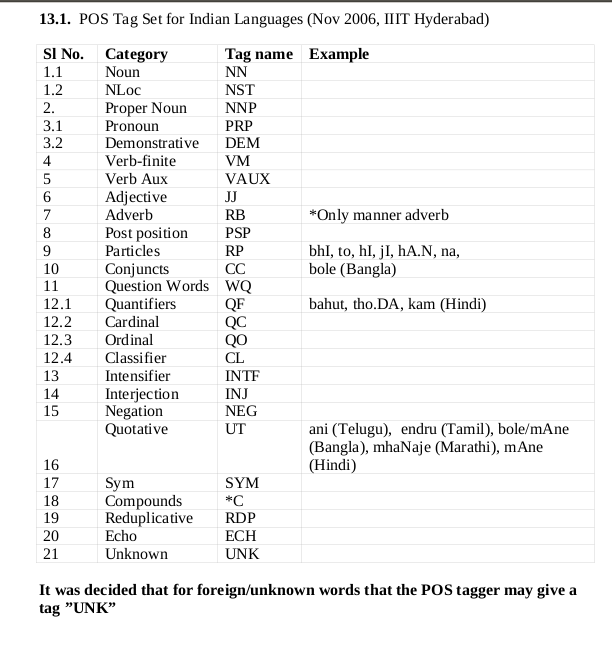
\includegraphics[width=0.7\textwidth]{poshindi.png}
\end{frame}

\begin{frame}
\frametitle{Tagged Reference Corpus}
\begin{itemize}
\item When they create tagsets, researchers also create a reference corpus of sentences which are manually annotated with these tags.
\item Annotation projects are usually long, time and money intensive, and lots of linguists work together.
\item Lots of guidelines, and manuals are prepared to make annotations unambiguous, and with good agreement between humans.
\item These tagged corpora are then used for developing automatic taggers.
\item So, important thing to keep in mind: there is no guarantee that the tagger will do well on unseen, out of domain data.
\end{itemize}
\end{frame}

\begin{frame}
\frametitle{POS Tagging: How?}
All approaches to tagging fall into one of the two categories: 
\begin{enumerate}
\item Rule based tagging
\item Probabilistic tagging
\end{enumerate}
There is something called "Transformation based Learning" which has features of both these methods.
\end{frame}

\begin{frame}
\frametitle{Rule based tagging}
This is usually a two stage process:
\begin{enumerate}
\item Stage 1: Assign all possible POS tags for a given word based on language dictionary.
\item Stage 2: Write linguistic disambiguation rules to choose one POS tag for that word in that context.
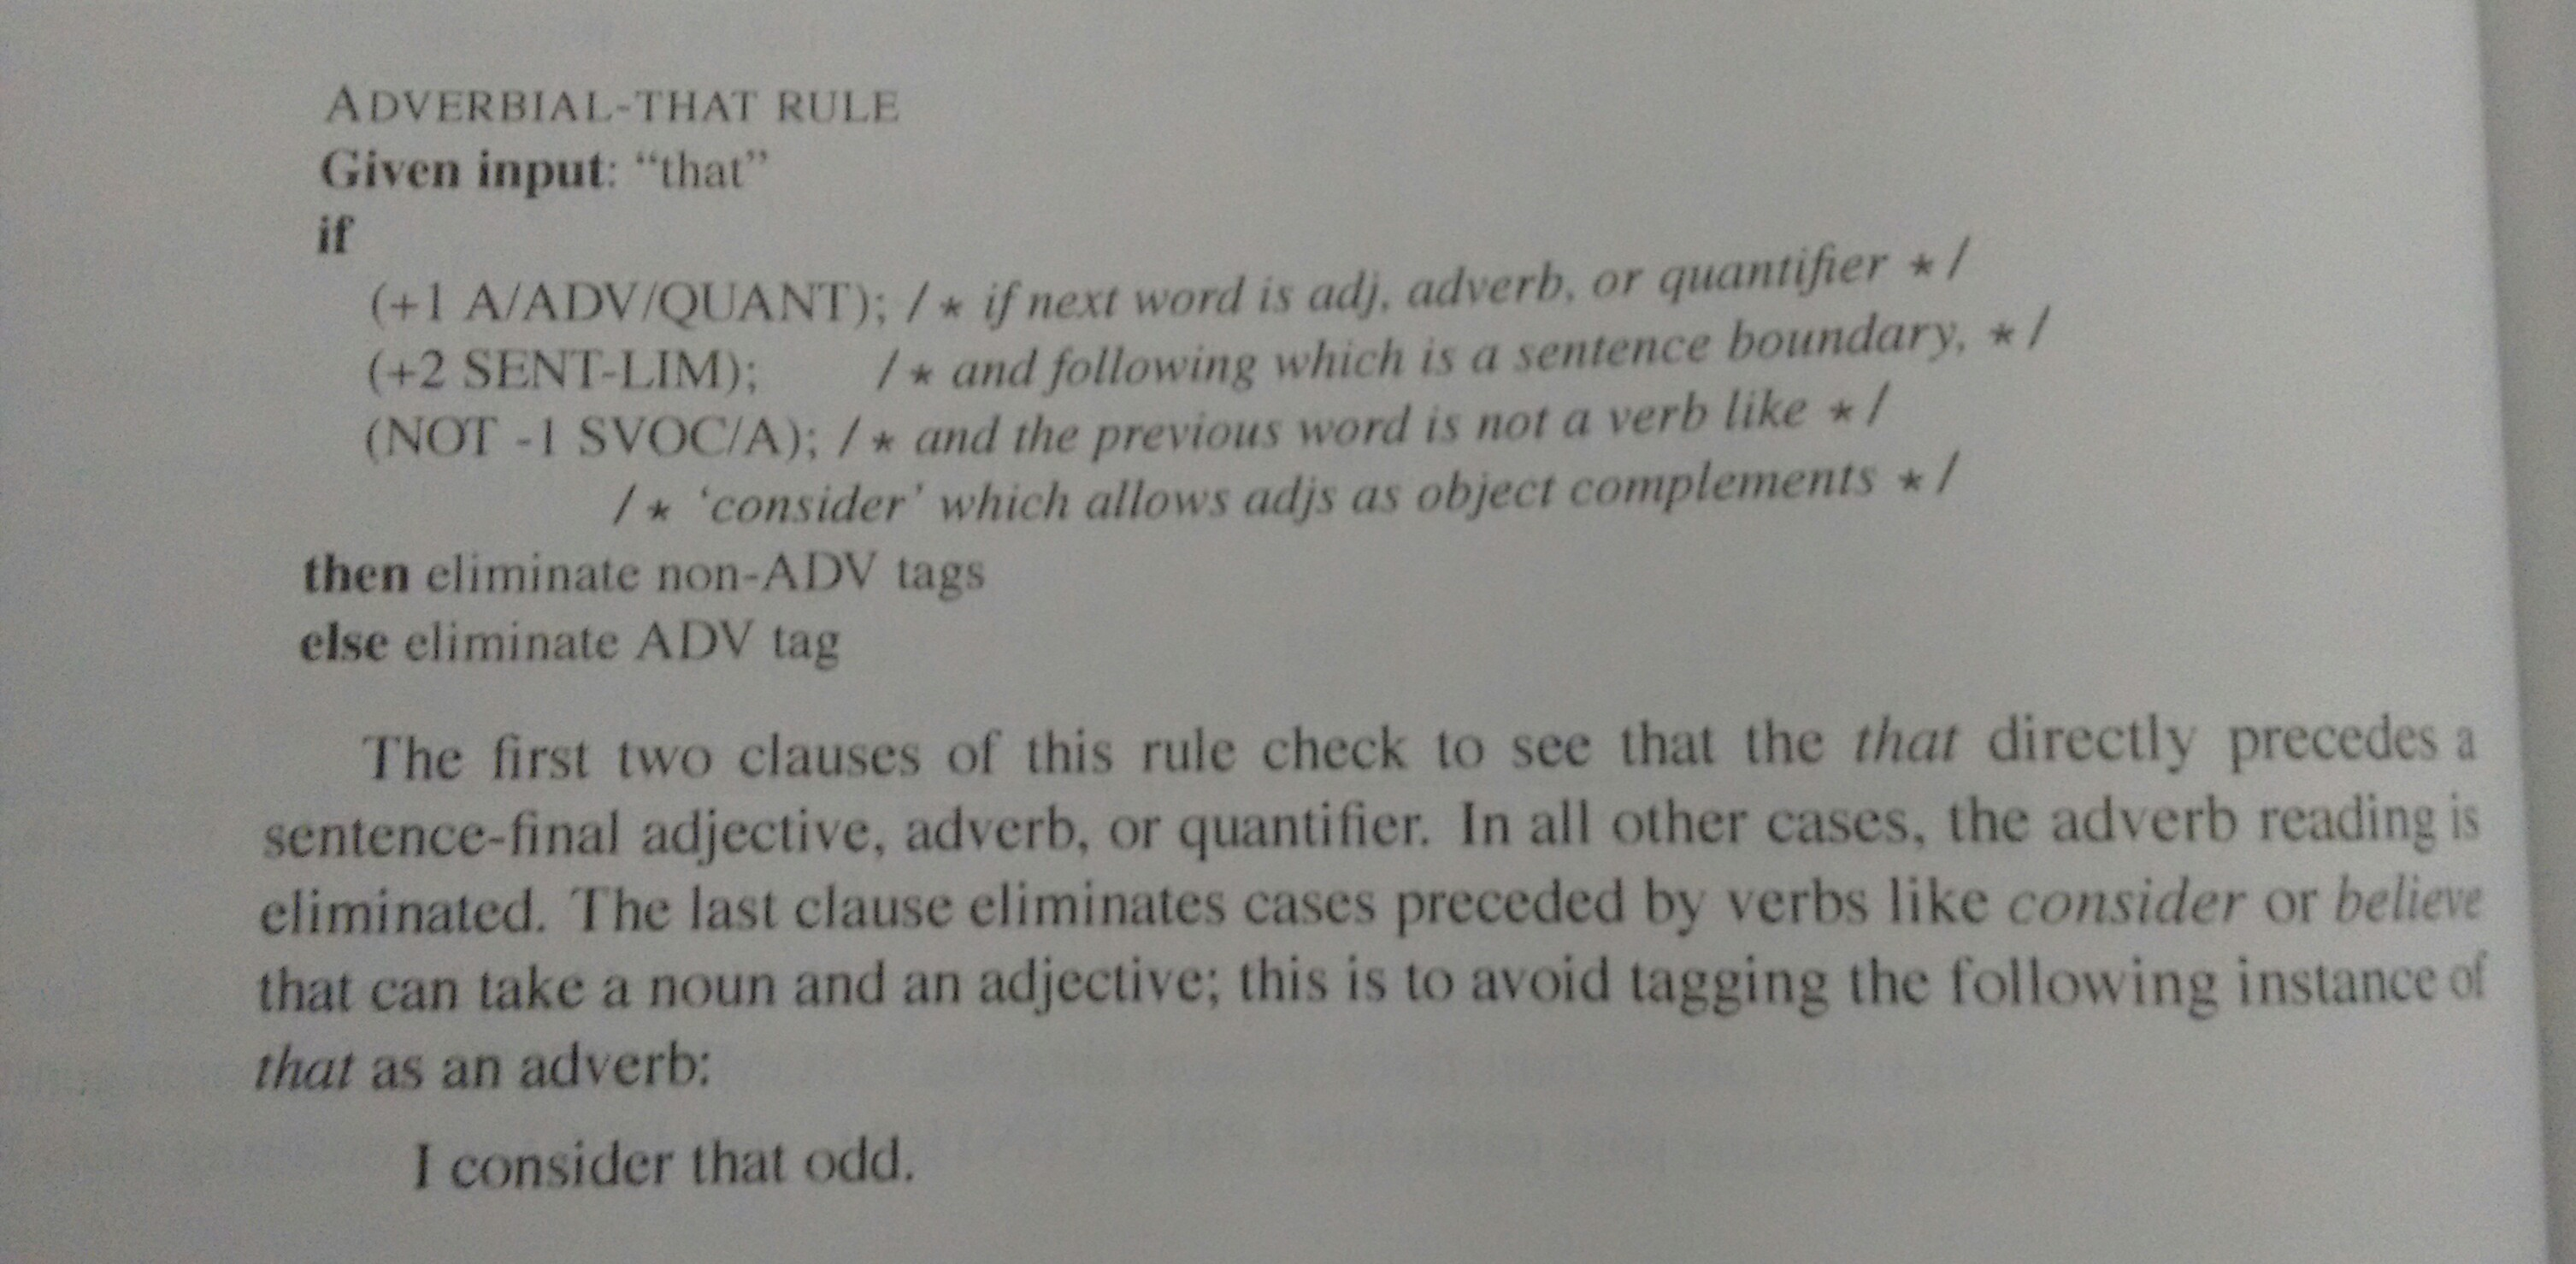
\includegraphics[width=0.9\textwidth]{POSRules.jpg}
\end{enumerate}
\end{frame}

\begin{frame}
\frametitle{Probabilistic Tagging - Background}
\begin{itemize}
\item POS tagging can be viewed in two ways: 
\begin{enumerate}
\item Text classification: Given some word, predict its most likely tag - classifying some text (word) into some pre-defined category (tag)
\item As sequence classification/labeling: given a sequence of words, predict the most likely sequence of tags.
\end{enumerate}
\item POS tagging is generally treated and modeled as sequence classification. 
\item Aim in modeling POS tagging as sequence labeling: given a sequence of n words, out of all possible sequences of n tags, choose the one that is most likely for that word sequence
\end{itemize}
\end{frame}

\begin{frame}
\frametitle{Sequence Labeling - Mathematical Notation}
\begin{itemize}
\item If w$_1^n$ is our sequence of n words,
\item ... and t$_1^n$ is the collection of all sequences of ntags
\item We should pick a tag sequence, so that P(t$_1^n|$w$_1^n$) is the highest.
\item $\hat t_1^n$ = argmax$_{t_1^n}$ P(t$_1^n|$w$_1^n$)
\item If we use this notation: argmax$_x$ f(x), it means "value of x such that f(x) is maximized".
\item So how do we find out P(t$_1^n|$w$_1^n$) first, to get its argmax value?
\end{itemize}
\end{frame}

\begin{frame}
\frametitle{When in trouble, ask Mr Bayes}
\begin{itemize}
\item P(t$_1^n|$w$_1^n$) = P(w$_1^n|$t$_1^n$)*P(t$_1^n$)/P(w$_1^n$)
\item So, $\hat t_1^n$ = argmax$_{t_1^n}$(P(w$_1^n|$t$_1^n$)*P(t$_1^n$)/P(w$_1^n$))
\item which is $\hat t_1^n$ = argmax$_{t_1^n}$(P(w$_1^n|$t$_1^n$)*P(t$_1^n$)) - how? why is the denominator dropped? \pause
\item Answer: We are doing argmax over tag sequence. That does not affect the word sequence probability. So, that will remain same in all comparisons for argmax.
\item Here, P(w$_1^n|$t$_1^n$) is the likelihood of the word string given a tag string and P(t$_1^n$) is the prior probability of a tag sequence.
\end{itemize}
\end{frame}

\begin{frame}
\frametitle{Assumptions we make in calculations}
\begin{itemize}
\item This equation $\hat t_1^n$ = argmax$_{t_1^n}$(P(w$_1^n|$t$_1^n$)*P(t$_1^n$)) suffers from the same problems as language models. So we make some assumptions to simplify our calculations again.
\item First assumption: probability of a word depends only on its POS tag, not on previous words or tags.
\\ $\Rightarrow$ \small{P(w$_1^n|$t$_1^n$)} \normalsize $\approx$ $\pi_{i=1}^n$ \small{P(w$_i|$t$_i$)} \normalsize
\item Second assumption: probability of a tag appearing is only dependent on previous tag instead of entire history (for Bigram taggers!)
\\ $\Rightarrow$ \small{P(t$_1^n$)} \normalsize $\approx$ $\pi_{i=1}^n$ \small{P(t$_i|$t$_{i-1}$)} \normalsize
\item Considering these assumptions, $\hat t_1^n$ becomes: argmax$_{t_1^n} \pi_{i=1}^n$(P(w$_i|$t$_i$)*P(t$_i|$t$_{i-1}$))
\end{itemize}
\end{frame}

\begin{frame}
\frametitle{What does all this mean in normal language?}
\begin{itemize}
\item This is the equation we have: \\ $\hat t_1^n$ = argmax$_{t_1^n} \pi_{i=1}^n$(P(w$_i|$t$_i$)*P(t$_i|$t$_{i-1}$))
\item (P(w$_i|$t$_i$) = Count(t$_i,w_i$)/Count(t$_i$)
\\ $\Rightarrow$ P(good$|$ADJ) = C(ADJ,good)/C(ADJ)
\item P(t$_i|$t$_{i-1}$) = Count(t$_{i-1},t_i$)/Count(t$_{i-1}$) (Same as in language models)
\\  $\Rightarrow$  P(NN$|$DT) = C(DT,NN)/C(DT)
\item This is HMM tagging. The "Hidden" here refers to the tag sequence, because that is something that we cannot observe in the input which is only a sequence of words.
\item If we use HMM for speech recognition, "observed" state is speech sequence, hidden state is word sequence.
\end{itemize}
Note: There is a lot of stuff about HMM I am not discussing here. Interested people - read Chapter 5 (and perhaps 6 too) in J\&M. It may need advance mathematical background.
\end{frame}

\begin{frame}
\frametitle{Assignment 3 Description}
\begin{itemize}
\item clarification regarding Q1: I am not expecting you to implement a HMM tagger (you can, if you want to). I am fine with seeing an implementation that is based on trigrams of the kind P(Tag2$|$(Tag1Word2))
\end{itemize}
\end{frame}

\begin{frame}
\frametitle{Practice Exercise -1}
Find one tagging error in each of the following sentences tagged with the PTB tagset. (Q 5.1 in J\&M)
\begin{enumerate}
\item I/PRP need/VBP a/DT flight/NN from/IN Atlanta/NN
\item Does/VBZ this/DT flight/NN serve/VB dinner/NNS
\item I/PRP have/VB a/DT friend/NN living/VBG in/IN Denver/NNP
\item Can/VBP you/PRP list/VB the/DT nonstop/JJ afternoon/NN flights/NNS
\end{enumerate}
note: PTB tags: \url{https://goo.gl/JVKbYM}
\end{frame}

\begin{frame}
\frametitle{Practice Exercise -2}
Chapter 5 of NLTK book is about POS tagging and how to use NLTK for that. Go to RegEx tagger description there, and try to develop a small regex tagger on your own, which identifies adjectives and verbs. Test it with some sentences and note your observations. Work in groups of 3. On tuesday, we will start with some presentations of this. 
\end{frame}

\begin{frame}
\frametitle{Practice Exercise - 3} 
Modify Katrin Erk's code sample to incorporate Laplace smoothing and return Log probabilities instead of normal probability.
\\Note: This is going to be useful in doing Question 1 of Assignment 3. So, try to do this.
\end{frame}

\begin{frame}
\frametitle{Next Class}
\begin{itemize}
\item Conclusion of POS tagging discussion: Transformation Based Learning, Evaluation of Taggers
\item ToDo: listen to Lectures 7.2-7.5 in Radev's coursera course.
\item Read and try to work through examples in Chapter 5 of NLTK (This will help you solve one question in A3)
\end{itemize}
\end{frame}
\end{document}


%Next time: TBL, Evaluating and comparing taggers - WER/TER stuff, comment on English tagger accuracy, acc. fr other languages. 
%Q 5.2 from J&M
